\begin{solution}
\begin{enumerate}
\item {[5 points]} Since $f(x) = 8x^2(1-x) = 8\left(x^2-x^3\right)$, we have that, for $k=1,2,\ldots$,
\begin{eqnarray*}
(f,\psi_k)&=&8\sqrt{2}\int_0^1 \left(x^2-x^3\right) \sin\left(k\pi x\right)\, dx
\\
&=&8\sqrt{2}\left(\left[-{1\over k\pi}\left(x^2-x^3\right)\cos\left(k\pi x\right)\right]_0^1+{1\over k\pi}\int_0^1 \left(2x-3x^2\right) \cos(k\pi x)\, dx\right)
\\
&=&{8\sqrt{2}\over k\pi}\int_0^1 \left(2x-3x^2\right) \cos(k\pi x)\, dx
\\
&=&{8\sqrt{2}\over k\pi}\left(\left[{1\over k\pi}\left(2x-3x^2\right)\sin\left(k\pi x\right)\right]_0^1-{1\over k\pi}\int_0^1 \left(2-6x\right) \sin(k\pi x)\, dx\right)
\\
&=&-{8\sqrt{2}\over k^2\pi^2}\int_0^1 \left(2-6x\right) \sin(k\pi x)\, dx
\\
&=&-{8\sqrt{2}\over k^2\pi^2}\left(\left[-{1\over k\pi}\left(2-6x\right)\cos\left(k\pi x\right)\right]_0^1-{6\over k\pi}\int_0^1 \cos(k\pi x)\, dx\right)
\\
&=&-{8\sqrt{2}\over k^2\pi^2}\left({4\over k\pi}\cos\left(k\pi\right)+{2\over k\pi}-{6\over k\pi}\left[{1\over k\pi}\sin(k\pi x)\right]_0^1\right)
\\
&=&{-16\sqrt{2}\over k^3\pi^3}\left(1+2\cos\left(k\pi\right)\right)
\\
&=&{-16\sqrt{2}\over k^3\pi^3}\left(1+2\left(-1\right)^k\right).
\end{eqnarray*}
Hence, the best approximation to $f$ from ${\rm span}\left\{\psi_1,\ldots,\psi_N\right\}$ with respect to the norm $\norm{\cdot}$ is
\begin{eqnarray*}
f_N(x)&=&\sum_{j=1}^N\ip{f,\psi_j}\psi_j(x)
\\
&=&\sum_{j=1}^N{-16\sqrt{2}\over j^3\pi^3}\left(1+2\left(-1\right)^j\right)\sqrt{2}\sin(j\pi x)
\\
&=&\sum_{j=1}^N{-32\over j^3\pi^3}\left(1+2\left(-1\right)^j\right)\sin(j\pi x).
\end{eqnarray*}
\\
\item {[6 points]}  The series solution that we obtain using the spectral method is
\[
u(x)= \sum_{j=1}^\infty {\ip{f,\psi_j} \over \lambda_j}\psi_j(x)=\sum_{j=1}^\infty{-32\over j^5\pi^5}\left(1+2\left(-1\right)^j\right)\sin(j\pi x).
\]
\\
The best approximation to $u$ from ${\rm span}\left\{\psi_1,\ldots,\psi_N\right\}$ with respect to the norm $\norm{\cdot}$ is
\[
u_N(x)=\sum_{j=1}^N{\ip{f,\psi_j} \over \lambda_j}\psi_j(x)=\sum_{j=1}^N{-32\over j^5\pi^5}\left(1+2\left(-1\right)^j\right)\sin(j\pi x).
\]

\item {[2 points]} The requested plot is below.

\begin{center}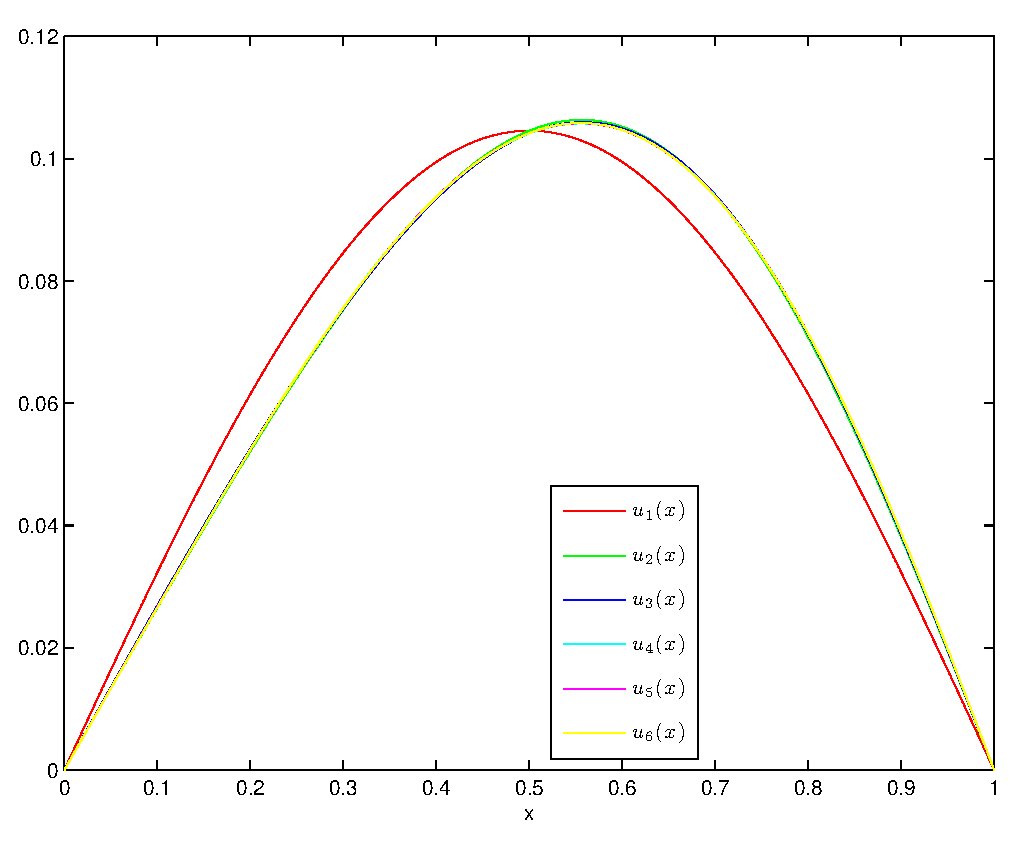
\includegraphics[scale=0.7]{hw26d.eps}\end{center}

The above plot was produced using the following MATLAB code.

\lstinputlisting{HW26d.m}

\item {[6 points]} Let $u$ be the solution to $Lu=f$ and let $w\in C^2[0,1]$ be such that
\[
-w''(x)=0,\quad0<x<1;
\]
\[
w(0)=-{1\over4}
\]
and
\[
w(1)={1\over4}.
\]
Then $\tilde{u}(x)=w(x)+u(x)$ will be such that
\[
-\tilde{u}''(x)=-w''(x)-u''(x)=0+f(x)=f(x);
\]
\[
\tilde{u}(0)=w(0)+u(0)=-{1\over4}+0=-{1\over4};
\]
and
\[
\tilde{u}(1)=w(1)+u(1)={1\over4}+0={1\over4}.
\]
Now, the general solution to
\[
-w''(x)=0
\]
is $w(x)=Ax+B$ where $A$ and $B$ are constants. Moreover, $w(0)=B$ and so $w(0)=-{1\over4}$ when $B=-{1\over4}$. Hence, $w(x)=Ax-{1\over4}$ and so $w(1)=A-{1\over4}$ and hence $w(1)={1\over4}$ when $A={1\over4}+{1\over4}={2\over4}={1\over2}$. Consequently,
\[
w(x)={1\over2}x-{1\over4}
\]
and so
\[
\tilde{u}(x)={1\over2}x-{1\over4}+u(x).
\]
We can then use the series solution to $Lu=f$ that we obtained in part (e) to obtain the series solution
\[
\tilde{u}(x)={1\over2}x-{1\over4}+\sum_{j=1}^\infty{-32\over j^5\pi^5}\left(1+2\left(-1\right)^j\right)\sin(j\pi x)
\]
to the problem of finding $\tilde{u}\in C^2[0,1]$ such that
\[
-\tilde{u}''(x)=f(x),\quad0<x<1;
\]
\[
\tilde{u}(0)=-{1\over4}
\]
and
\[
\tilde{u}(1)={1\over4}.
\]
\\
\item {[2 points]} The requested plot is below.

\begin{center}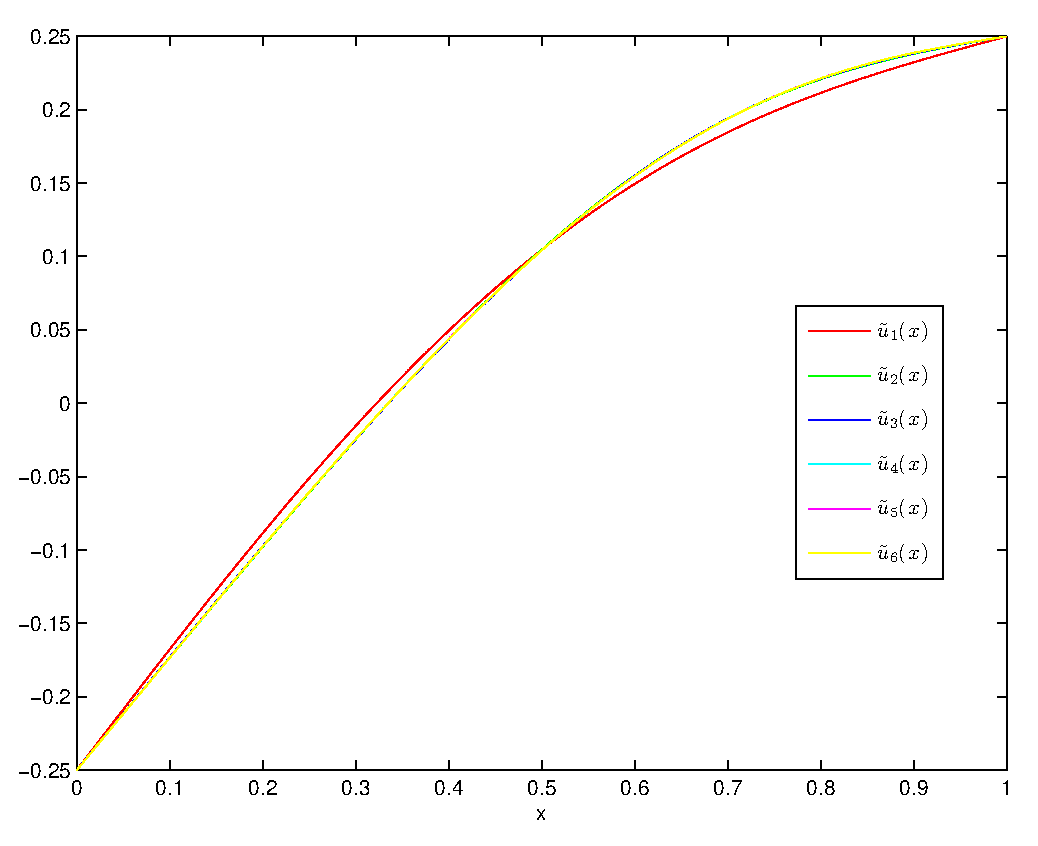
\includegraphics[scale=0.7]{hw26g.eps}\end{center}

The above plot was produced using the following MATLAB code.

\lstinputlisting{HW26g.m}

\end{enumerate}

\end{solution}

